% !TEX root =  ../main.tex
\section{Fence}
\subsection{Definition}

\subsubsection{Signature} \cstr{fence(s1 : set<VM>, s2 : set<server>)}

\begin{itemize}
\item \cstr{s1} : an non-empty set of VMs for a meaningful constraint. VMs not in the \st{Running} state are ignored.
\item \cstr{s2} : an non-empty set of servers or the constraint is sure of not being satisfiable.
Servers not in the \st{Online} state are ignored.
\end{itemize}

The \cstr{fence} constraint forces each running VM in \cstr{s1} to be running on one of
the online servers in \cstr{s2}. 

\classification{fence}{datacenter administrator}{VM placement}{Partitioning,VM-to-server placement}

\subsubsection{Usage}

A \cstr{fence} constraint deserves partitioning purposes. First, it may be used by a datacenter administrator to part the infrastructure. Such a situation is typically motivated for security or administrative purposes. As an example, a datacenter may be the property of multiple organizations that have aggregated their servers. However, administrative policies may disallow to have specific VMs of one organization running on servers belonging to another organization. In this setting, \cstr{fence} constraints may be used to specify the list of allowed servers for these VMs.

Another possible usage of \cstr{fence} constraints consist in splitting the VMs when the infrastructure is designed using an aggregation of independent partitions of servers. As an example, a partition may consist of a standalone shipping container of servers or all the servers connected to a same storage space when VMs disk images are only available to these servers. In this setting, \cstr{fence} constraint allow the datacenter administrator to restrict the placement of the VMs to their assigned partition.

Finally, a \cstr{fence} constraint may be used as a backend for a resource matchmaking
system~\cite{condor-classad} for non-cumulative resources. As an example, a VM may require a particular
hypervisor, processor or GPU. \cstr{Fence} constraints may then be used to force the VMs to be running on compatible environments. The list of the compatible servers must be established before using the constraint. It has to be noticed that this use case is not suitable when the matchmaking is focusing shareable but finite resources such as memory or computing power.


\subsubsection{Example}

Figure~\ref{fig: fence} depicts a sample reconfiguration between a source and a destination configuration. In this example, the following \cstr{fence} constraints were considered.
\begin{itemize}

\item \cstr{fence(\{VM1,VM2\}, \{N1, N2\})}. This constraint was already satisfied in the source configuration as both VMs were running on \cstr{N1}. The constraint is still satisfied in the destination configuration despite \cstr{VM2} has been relocated to \cstr{N2} as this action is allowed by the constraint.

\item \cstr{fence(\{VM2, VM3\}, \{N2\})}. This constraint was not satisfied in the source configuration as \cstr{VM2} was not running on \cstr{N2}. Its relocation to \cstr{N2} during the reconfiguration fixed this violation. During the reconfiguration process, \cstr{VM3} has been stopped and is now in the \st{Waiting} state. The VM was then ignored by the constraint.
\end{itemize}

\begin{reconfiguration}
\centering
\begin{minipage}[b]{0.40\textwidth}
\begin{lstlisting}
N1: VM1 VM2
N2: VM3
N3:
?: VM4
\end{lstlisting}
\end{minipage}
\begin{minipage}[b]{2cm}
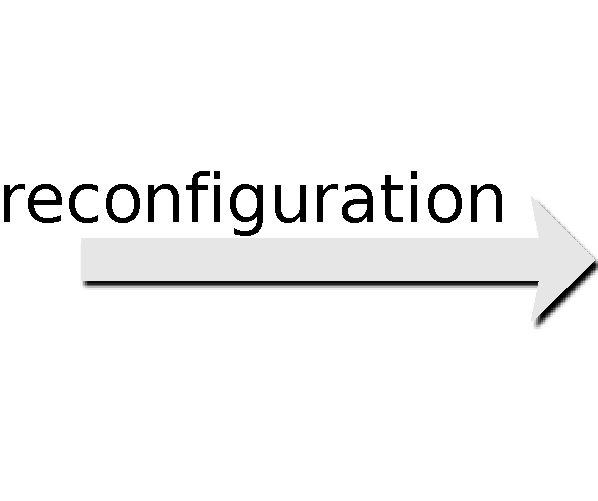
\includegraphics[width=2cm]{img/arrow_reconfiguration}
\end{minipage}
\begin{minipage}[b]{0.40\textwidth}
\begin{lstlisting}
N1: VM1 VM4
N2: VM2
N3:
?: VM3
\end{lstlisting}
\end{minipage}
\caption{A reconfiguration motivated by \cstr{fence} constraints.}\label{fig: fence}
\end{reconfiguration}

\fullVersion{
\subsection{Model}

The \cstr{fence} constraint is modeled using a domain restriction on the demanding slice associated to each of the running VMs to force each placement variable to take its value inside the values denoting
the allowed servers.

\begin{equation*}
\begin{split}
\text{\cstr{fence}}&\text{\cstr{(V : set<VM>, N : set<server>)}} \triangleq\\
 & d_i^h \in \{\forall j | n_j \in N\}, \forall v_i \in V
\end{split}
\end{equation*}

\subsection{Violation Detection}

The detection of the violating elements in \cstr{fence} consists in identifying the VMs that are not hosted
on the allowed servers. The computed selection of misplaced VMs is necessary minimal with regards to the scope of the constraint.

\subsection{Availability}

\subsubsection{In {\btrp}} This constraint is available using the name \texttt{Fence}. Using the global constraint catalog~\cite{gccat}, the domain of the d-slice placement variable is restricted to the values
denoting the allowed servers using a \emph{in} constraint. Using Choco, the domain of the variable is
directly filtered. The following denotes the model based on the global constraint catalog:

\begin{equation*}
\begin{split}
\text{\cstr{fence}}&\text{\cstr{(V : set<VM>, N : set<server>)}} \triangleq\\
	& in(d_i^h, \{\forall j | n_j \in N\}), \forall v_i \in V
\end{split}
\end{equation*}

\subsubsection{In VMWare}
}

\subsection{See also}

\subsubsection{Related Constraints}
\begin{itemize}
\item \cstrref{ban}: the opposite constraint of \cstr{fence}.
One \cstr{fence} constraint can be emulated using a \cstr{ban} constraint by specifying to the \cstr{ban} 
constraint the absolute complement of the set of servers specified in the \cstr{fence} constraint.

\item \cstrref{quarantine}: This constraint encapsulates the \cstr{fence} constraint but also disallows the VMs outside the fence to be relocated to servers inside the fence.

\item \cstrref{among}: The \cstr{among} constraint encapsulates the \cstr{fence} constraint.
The given VMs will necessarily be running on a single set of servers but multiple candidate set of servers may be passed as an argument to let the \cstr{among} constraint state about the set of servers to choose. A \cstr{fence} constraint can be emulated using one \cstr{among} constraint when only of set of servers is specified.
\end{itemize}

\emulatedWith{fence}{ban}{\cstr{fence(vs1, ns1)}}{\cstr{ban(vs1,\oline{ns1})}}
\printListOfInheritance{fence}